%*****************************************
\chapter{Introduzione}\label{ch:introduction}

Negli ultimi anni molte branche della scienza e dell'industria si trovano a produrre e analizzare insiemi di dati sempre più grandi e complessi. Questi Big Data sono difficilmente analizzabili usando tecniche standard a causa di problemi sia tecnici che teorici.

Ad esempio, dover processare grandi quantità di dati complessi può avere facilmente un costo troppo elevato in termini di tempo e memoria rispetto alle possibilità della tecnologia odierna. Vi sono poi problemi che si annidano nell'analisi di dati in elevate dimensioni, in cui bisogna tenere conto di alcune particolarità, come il fatto che la distanza fra due punti smette di essere significativa.

Si può visualizzare questa cosa confrontando l'estrazione casuale di punti dal quadrato in dimensione 2 o dall'ipercubo in dimensione 100: estratti due punti $x$ e $y$ dalla distribuzione uniforme sull'ipercubo unitario in $\R^d$, la distanza fra loro è
\begin{equation*}
  d(x,y) = \sqrt{\sum_{i=1}^d (x_i - y_i)^2},
\end{equation*}
allora per la disuguaglianza di Hoeffding la distribuzione di $d(x,y)$ è concentrata attorno al valore medio per dimensioni $d$ elevate. In \cref{fig:pointdistance} si può vedere la differenza: i due grafici mostrano l'andamento della distanza di un punto casuale dell'ipercubo da altri 100 punti casuali per $d=2$ e $d=100$. Si può notare come all'aumentare della dimensione i valori si schiacciano attorno al valor medio.

\begin{figure}[ht]
  \begin{center}
    \begin{subfigure}[b]{.4\textwidth}
      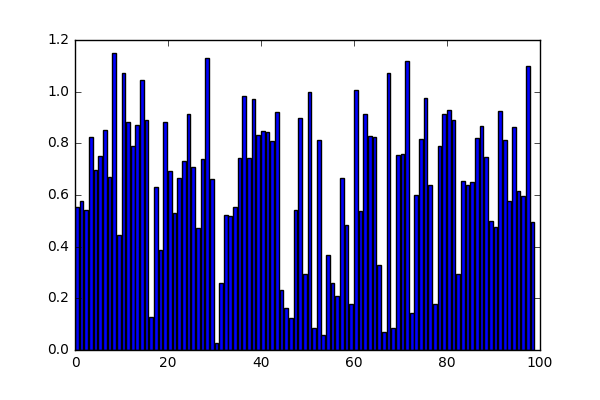
\includegraphics[width=\textwidth]{gfx/pltpoints2d.png}
      \caption{$d=2$}
    \end{subfigure}
    \begin{subfigure}[b]{.4\textwidth}
      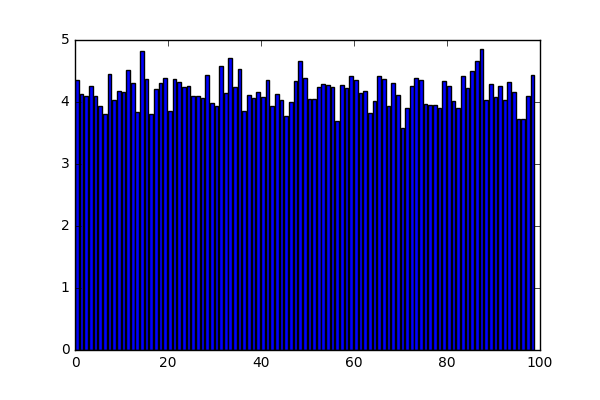
\includegraphics[width=\textwidth]{gfx/pltpoints100d.png}
      \caption{$d=100$}
    \end{subfigure}
    \caption{Distanza fra punti casuali nell'ipercubo}  \label{fig:pointdistance}
  \end{center}
\end{figure}

Ci interessa quindi sviluppare tecniche in grado di rivelare informazioni in spazi metrici di dimensione possibilmente elevata, in particolare vorremmo poter riassumere in un numero finito (piccolo) di variabili l'informazione che ci serve.

Utilizzeremo tecniche topologiche, e le informazioni che queste ci consentiranno di catturare riguardano la \emph{forma} dei dati. In dimensioni elevate è difficile visualizzare un insieme di punti e quindi comprendere se questo abbia una forma interessante, tuttavia utilizzando la topologia è possibile produrre una rappresentazione sintetica di uno spazio complesso mediante una quantità finita di informazioni, e tale che calcolando opportuni invarianti di questa rappresentazione si ricavino informazioni sulla \emph{forma} dello spazio. La topologia consente anche di esprimere mediante quantità precise cosa intendiamo per \emph{forma}.
